\documentclass[10pt,twocolumn]{article}
\usepackage[a4paper,margin=1.9cm,columnsep=0.7cm]{geometry}
\usepackage[T1]{fontenc}
\usepackage{newtxtext,newtxmath}
\usepackage{microtype}
\usepackage{graphicx}
\usepackage{booktabs}
\usepackage{tabularx}
\usepackage{amsmath}
\usepackage{enumitem}
\usepackage{xcolor}
\usepackage[font=small,labelfont=bf]{caption}
\usepackage[hidelinks]{hyperref}
\usepackage{url}
\setlist{nosep,leftmargin=*}
\newcommand{\pred}[1]{\texttt{#1}}
\newcommand{\suite}[1]{\texttt{#1}}
\graphicspath{{figures/}}

\title{\textbf{When Does a Simulated Success Hold?\\ Auditing LIBERO's Success Predicates on 2{,}000 Demonstrations}}
\author{Author names and affiliations to be added}
\date{Draft of 11 November 2026}

\begin{document}
\maketitle

\begin{abstract}
Simulated manipulation benchmarks report success rates computed by hand-written predicates, and those rates are used to rank policies. Whether a predicate's verdict describes a completed task is rarely examined. We audit the success predicates of LIBERO, one of the most widely used benchmarks, using only material the benchmark itself distributes: its checker source, its 40 task definitions and its 2{,}000 human demonstrations. The checker evaluates the goal on every control step and ends the episode at the first step on which it holds; none of its predicates requires the object to be at rest, to be released, or to stay in place. Of the 50 goal predicates across the 40 tasks, 44 are \pred{On} or \pred{In}, and all 20 \pred{In} goals target a region for which the contact test is unconditionally true. We restore the final logged state of every demonstration in the simulator and continue for 5\,s under two post-success protocols. With the gripper held, 18 of 2{,}000 benchmark-accepted successes (0.90\%, task-clustered 95\% interval 0.30--1.65\%) no longer satisfy the predicate; with the gripper released, 75 do (3.75\%, 0.40--9.40\%). The loss is concentrated: one task accounts for 63\% of it and five tasks for 95\%. In that task the predicate holds while the object is carried above its goal compartment and fails once the object stands inside it, which we confirm in renders. Independently of the outcome, the predicate turns false at least once after first turning true in 30\% of demonstrations, and in 48\% of those with an \pred{On} goal. Predicate error on LIBERO is thus small on average but task-specific and large where it occurs; a consecutive-step persistence window is a poor strict grader; and intervals that treat episodes as independent understate uncertainty several-fold when errors cluster by task. All verdicts in this paper are referenced to the simulator; policy rollouts and human labels are left to future work.
\end{abstract}

\section{Introduction}

A success rate on a simulated benchmark is a count of episodes on which a predicate returned true. The predicate is a few lines of code written once by the benchmark's authors. Every published number inherits its definition, and so does every ranking built on those numbers.

Recent audits have questioned what such benchmarks measure. They report that small probes solve tasks without language, that many claimed improvements are not statistically significant, and that modest perturbations collapse performance \cite{jiang2026benchmarking,zhou2025liberopro,fei2025liberoplus}. These studies take the success predicate as given. A complementary line of work shows that simulators can eject correctly placed objects, so that a failure is the simulator's fault and not the policy's \cite{zhou2026simuguard}. The predicate itself, the component that turns a physical state into a verdict, has received less scrutiny.

We ask a narrow question that can be answered without training or running any policy: \emph{when LIBERO's own checker accepts an episode, does the accepted state persist?} We answer it on the 2{,}000 human demonstrations that LIBERO distributes \cite{liu2023libero}. These are the cleanest successes the benchmark has: each was produced by a person and accepted by the checker. If verdicts are fragile here, they are fragile for a reason that lies in the checker and not in any policy.

\paragraph{Contributions.}
\begin{enumerate}
\item A code-level description of when and how LIBERO declares success, and a taxonomy of the goal predicates of all 40 tasks in its four standard suites (Sections~\ref{sec:background} and~\ref{sec:taxonomy}).
\item A replay protocol that restores logged simulator states exactly and extends each episode under a stated post-success protocol, together with two failure modes of such harnesses that produce spurious results if left uncorrected (Section~\ref{sec:replay}).
\item Measurements on 2{,}000 demonstrations of how often an accepted success is lost within 5\,s, how often the predicate flickers, and how both distribute over tasks and predicate types, with intervals that respect clustering by task (Section~\ref{sec:results}).
\item A concrete predicate defect in one task, where the goal is satisfied while the object is carried and not once it rests (Section~\ref{sec:book}).
\item Open analysis code with derivations for every estimator.
\end{enumerate}

\paragraph{Scope of this version.} The study uses demonstrations only. It contains no policy rollouts and no human labels, and it covers one benchmark. Section~\ref{sec:limits} states what follows from that.

\section{Related Work}

The positioning in this section rests on the abstracts of the cited papers, and for \cite{jiang2026benchmarking} also on its project page; it must be re-checked against the full texts before submission.

\paragraph{Benchmark validity.} Jiang et al.\ \cite{jiang2026benchmarking} audit LIBERO, CALVIN, SimplerEnv, RoboCasa \cite{nasiriany2024robocasa} and RoboTwin~2.0 for shortcut solvability, statistical significance, creeping overfitting and data-source dependence. LIBERO-PRO \cite{zhou2025liberopro} and LIBERO-Plus \cite{fei2025liberoplus} perturb objects, initial states, instructions, cameras and lighting and report large drops for models that exceed 90\% on the standard suites. All three measure what a success rate fails to capture about the policy. None, as far as their abstracts state, examines whether the predicate that defines success is itself correct.

\paragraph{Predicates.} LIBERO-X \cite{wang2026liberox} extends LIBERO and adds stricter predicates (\pred{ExactIn}, \pred{UprightOn}, \pred{SideOn}), which indicates that its authors found the originals too permissive; we have not yet verified whether it quantifies the difference. MANGO \cite{valle2026mango} generates test oracles automatically to replace hand-written symbolic ones and notes that such oracles judge only end states. Our work is complementary: it measures the existing oracle, and finds that in LIBERO the oracle is in fact not an end-state check but a first-hit check.

\paragraph{Simulator-caused failures.} SimuGuard \cite{zhou2026simuguard} is the closest neighbour. It instruments LIBERO, RoboTwin, RoboCasa and RoboDojo at every physics step and flags objects ejected by contact artifacts, attributing those failures to the simulator. It addresses false failures caused by physics. We address the verdict logic, in both directions, and our flicker measurements concern the same contact machinery from the predicate's side.

\paragraph{Success beyond the binary.} SafeVLA-Bench \cite{fan2026safevla} re-grades successful episodes against safety invariants and reports a success-but-unsafe rate. Bedi \cite{bedi2026silent} studies how observable false successes are in two bimanual simulation tasks with induced failures. FailBench \cite{navasardyan2026failbench} evaluates vision-language models as judges of task success, with a best mean balanced accuracy of 0.77. Episodes with verified outcomes are the kind of test set such judges need.

\paragraph{Position.} To our knowledge, no prior work reports how often a benchmark-accepted success in LIBERO fails to persist, or how that quantity distributes over tasks and predicate types.

\section{Background: How LIBERO Decides Success}
\label{sec:background}

All statements in this section were read from the \texttt{master} branch of the LIBERO repository on 10 November 2026.

\paragraph{When.} The environment's \texttt{step} function overwrites the termination flag with the goal check on every control step (\texttt{done = self.\_check\_success()}). An evaluation loop that stops on \texttt{done} therefore grades by \emph{first hit}: an episode counts as a success if the goal holds on any single step.

\paragraph{What.} A task goal is a conjunction of atomic predicates written in BDDL. Table~\ref{tab:predicates} gives their definitions. For a region, the contact test returns true unconditionally; the source comments that sites have no dynamics. \pred{In}$(a,r)$ with a region $r$ therefore reduces to a box test on one point of the object.

\begin{table}[t]
\centering\small
\caption{Atomic goal predicates as implemented in LIBERO. None has an at-rest, release or persistence condition.}
\label{tab:predicates}
\begin{tabularx}{\columnwidth}{@{}lX@{}}
\toprule
Predicate & Definition in the source \\
\midrule
\pred{In}$(a,b)$ & $b$ is in contact with $a$, and the body origin of $a$ lies inside the containment box of $b$ \\
\pred{On}$(a,b)$, $b$ an object & $a$ and $b$ are in contact, the horizontal distance of their body origins is below 0.03\,m, and the origin of $b$ is not above that of $a$ \\
\pred{On}$(a,r)$, $r$ a region & $a$ is within the region's footprint and in contact with the region's parent object \\
\pred{Open}, \pred{Close}, \pred{Turnon}, \pred{Turnoff} & Threshold on a joint position \\
\bottomrule
\end{tabularx}
\end{table}

\paragraph{Demonstrations are graded more strictly than rollouts.} The collection script ends a demonstration only after the goal has held for 10 consecutive steps. A policy rollout needs one. The benchmark thus applies a persistence requirement to its training data that it does not apply to evaluation.

\paragraph{Released data.} Each task file holds 50 demonstrations with actions, flattened MuJoCo states and the full model description. The \texttt{rewards} and \texttt{dones} arrays are written as zeros with a single one on the last step, so the files contain no per-step record of the predicate.

\section{Method}

\subsection{Data}
We use the official demonstration files of the four standard suites, \suite{libero\_spatial}, \suite{libero\_object}, \suite{libero\_goal} and \suite{libero\_10}: 40 tasks, 50 demonstrations each, 2{,}000 in total. No demonstration was excluded.

\subsection{Static taxonomy}
We parse the goal section of each of the 40 task definitions and record every atomic predicate with its arguments. A task's \emph{predicate class} is the set of predicate types in its goal.

\subsection{Terminal-state screening}
A logged state is the vector (time, generalised positions, generalised velocities). We recover the slot of each joint from the model description stored with the demonstration, using MuJoCo's ordering: bodies depth-first, a body's joints before those of its children, 7 position and 6 velocity entries for a free joint, one each for a hinge or slide. The recovered sizes are checked against the logged width for every demonstration; on \suite{libero\_goal} they give $1+41+37=79$, the logged width. For each goal object with a free joint we take the norms of its linear and angular velocity over the final 10 logged states and call the object \emph{moving} if either exceeds 0.01\,m/s or 0.10\,rad/s. This step needs no simulator.

\subsection{Extended replay}
\label{sec:replay}
For each demonstration we (A) load every logged state into the simulator and evaluate the goal on it, which yields the per-step predicate trace the files lack, and (B) restart from the exact last logged state and simulate 100 further control steps (5\,s at 20\,Hz), evaluating the goal after each. Two post-success protocols are run separately. Under \textbf{hold}, the motion command is zero and the gripper command of the last demonstration step is repeated. Under \textbf{release}, the gripper is commanded open with no motion for 20 steps, after which the arm retreats upward.

Two harness errors had to be removed before the results were stable. Both would affect any study that restores simulator states.
\begin{enumerate}
\item \emph{Stale controller state.} Restoring a simulator state does not update the end-effector pose cached by the operational-space controller, so the first command drives the arm toward the pose it had at reset. Before the fix, 26 of 50 opened drawers and 27 of 50 turned stove knobs appeared to lose their success; after refreshing the controller and resetting its goal, none did.
\item \emph{Open-loop replay drift.} Replaying the logged actions from the first logged state does not reproduce the logged states under our simulator versions, and 21 of 500 \suite{libero\_goal} replays never satisfy the goal. We therefore never regenerate states by replay; step (B) starts from the logged state itself.
\end{enumerate}
Software: LIBERO at \texttt{master}, robosuite 1.4.0, MuJoCo 3.2.3, Python 3.8. The recording versions are not documented in the files.

\subsection{Graders}
Let the trace be the predicate on the logged states followed by the predicate on the 100 extension steps. \textbf{G0} (first hit, the benchmark's rule) is true if the predicate is true on at least one step. An episode is \textbf{lost} if G0 is true and the predicate is false on the last extension step. It shows \textbf{flicker} if the predicate is false on at least one step after its first true step. \textbf{G1-$N$} (persistence) is true if the predicate holds on $N$ consecutive steps, $N\in\{10,30,100\}$. ``Lost'' is a false success with the simulator's own predicate after 5\,s as reference; it is not a human judgment.

\subsection{Statistics}
For $k$ events in $n$ episodes we report the Clopper--Pearson interval \cite{clopper1934}, whose limits are beta quantiles,
\begin{align}
p_L &= B^{-1}\!\left(\tfrac{\alpha}{2};\,k,\,n-k+1\right), \nonumber\\
p_U &= B^{-1}\!\left(1-\tfrac{\alpha}{2};\,k+1,\,n-k\right).
\end{align}
It assumes independent episodes. Demonstrations of one task share scene, objects and goal, so for every pooled rate we also report a percentile bootstrap interval that resamples whole tasks with replacement (5{,}000 resamples, fixed seed) \cite{davison1997}. Where the two disagree, the task-clustered interval is the one to rely on. Concentration is the share of all lost successes that falls in the $k$ tasks with the most, against $k/40$ under an even spread.

With zero events the exact upper limit has the closed form $p_U = 1-(\alpha/2)^{1/n}$, which fixes the sample a null claim needs: at the 95\% level, $n=200$ gives 1.83\%, and $n=368$ is the smallest $n$ that bounds the rate below 1\%.

All analysis is implemented in base MATLAB without toolboxes and covered by 23 unit tests whose expected values were computed independently.

\section{Results}
\label{sec:results}

\subsection{Taxonomy: 88\% of goal predicates carry no stability condition}
\label{sec:taxonomy}
The 40 tasks contain 50 atomic goal predicates (Table~\ref{tab:taxonomy}). 44 of them are \pred{On} or \pred{In}, and 38 of the 40 tasks contain at least one of the two. \suite{libero\_spatial} consists of ten \pred{On} goals and \suite{libero\_object} of ten \pred{In} goals; \suite{libero\_10} has nine composite goals out of ten. Every \pred{In} goal targets a region, for which the contact condition is vacuous.

\begin{table}[t]
\centering\small
\caption{Goal predicates of the 40 tasks.}
\label{tab:taxonomy}
\begin{tabular}{@{}lccc@{}}
\toprule
Predicate & Goal predicates & Tasks & Region targets \\
\midrule
\pred{On} & 24 & 21 & 7 \\
\pred{In} & 20 & 17 & 20 \\
\pred{Turnon} & 3 & 3 & 0 \\
\pred{Close} & 2 & 2 & 0 \\
\pred{Open} & 1 & 1 & 0 \\
\midrule
Total & 50 & 40 & 27 \\
\bottomrule
\end{tabular}
\end{table}

\subsection{Screening: accepted demonstrations end in motion}
Of the 1{,}900 demonstrations whose goal involves a free object, the object is moving at some point in the final 10 logged steps in 1{,}775 (93.4\%) and at the last logged state in 817 (43.0\%); Table~\ref{tab:screening} gives the split by suite. Because the predicate had already held for about 10 steps by then, the checker fires during placement, not after settling. Motion at acceptance does not by itself predict a lost success: in \suite{libero\_goal}, pushing the plate shows motion at the last state in 43 of 50 demonstrations and loses none.

\begin{table}[t]
\centering\small
\caption{Motion of the goal object at the end of accepted demonstrations.}
\label{tab:screening}
\begin{tabular}{@{}lccc@{}}
\toprule
Suite & Free object & Moving, last 10 steps & Moving, last state \\
\midrule
\suite{spatial} & 500 & 456 & 148 \\
\suite{object} & 500 & 500 & 263 \\
\suite{goal} & 400 & 361 & 141 \\
\suite{10} & 500 & 458 & 265 \\
\bottomrule
\end{tabular}
\end{table}

\subsection{Durability: few successes are lost, and the protocol matters four-fold}
All 2{,}000 demonstrations satisfy the goal on their logged states, on between 5 and 40 steps (median 11), consistent with the 10-step acceptance rule. Table~\ref{tab:overall} reports what remains after 5\,s of further simulation. With the gripper held, 0.90\% of accepted successes are lost; with the gripper released, 3.75\%.

\begin{table}[t]
\centering\small
\caption{Outcome of 2{,}000 accepted demonstrations after a 5\,s extension. Rates in percent with 95\% intervals: exact (episodes independent) and task-clustered bootstrap.}
\label{tab:overall}
\begin{tabularx}{\columnwidth}{@{}l>{\raggedright\arraybackslash}X>{\raggedright\arraybackslash}X@{}}
\toprule
Measure & Release & Hold \\
\midrule
Lost & 75 (3.75) & 18 (0.90) \\
\quad exact & [2.96, 4.68] & [0.53, 1.42] \\
\quad clustered & [0.40, 9.40] & [0.30, 1.65] \\
Flicker & 592 (29.6) & 540 (27.0) \\
\quad clustered & [21.9, 37.7] & [19.6, 34.6] \\
Fails G1-10 & 0 & 0 \\
Fails G1-30 & 58 (2.90) & 14 (0.70) \\
Fails G1-100 & 111 (5.55) & 59 (2.95) \\
\quad clustered & [2.00, 11.00] & [1.65, 4.35] \\
\bottomrule
\end{tabularx}
\end{table}

\begin{figure}[t]
\centering
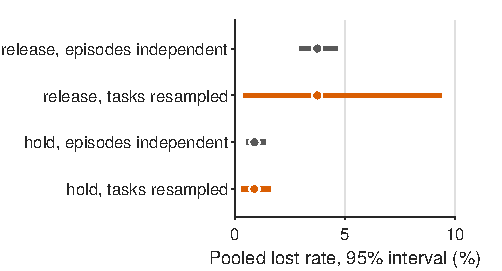
\includegraphics[width=\columnwidth]{fig_intervals.pdf}
\caption{The pooled lost rate with its two 95\% intervals. Treating the 2{,}000 episodes as independent gives an interval about five times narrower than resampling the 40 tasks does under the release protocol.}
\label{fig:intervals}
\end{figure}

For the release protocol the exact interval is about five times narrower than the task-clustered one (Fig.~\ref{fig:intervals}). The exact interval answers a question about 2{,}000 exchangeable episodes; the data are 40 tasks.

Table~\ref{tab:class} splits the result by suite and by predicate class. For pure \pred{On} goals a benchmark-accepted demonstration is durable: about 0.5\% are lost under either protocol. For \pred{In} goals the answer depends on whether the gripper lets go.

\begin{table}[t]
\centering\small
\caption{Lost successes by suite and by goal-predicate class, and flicker by class (release).}
\label{tab:class}
\begin{tabular}{@{}lrrrr@{}}
\toprule
 & $n$ & Lost, rel. & Lost, hold & Flicker \\
\midrule
\suite{spatial} & 500 & 1 & 4 & 277 \\
\suite{object} & 500 & 2 & 0 & 39 \\
\suite{goal} & 500 & 3 & 1 & 133 \\
\suite{10} & 500 & 69 & 13 & 143 \\
\midrule
\pred{On} (19 tasks) & 950 & 4 & 5 & 452 \\
\pred{In} (15) & 750 & 49 & 3 & 100 \\
\pred{Close}+\pred{In} (2) & 100 & 20 & 9 & 20 \\
\pred{On}+\pred{Turnon} (2) & 100 & 2 & 1 & 20 \\
\pred{Open} (1) & 50 & 0 & 0 & 0 \\
\pred{Turnon} (1) & 50 & 0 & 0 & 0 \\
\bottomrule
\end{tabular}
\end{table}

\subsection{Concentration: one task carries 63\% of the loss}
Under release, the task with the most lost successes holds 62.7\% of all 75, the top three 89.3\% and the top five 94.7\%; an even spread would give 2.5\%, 7.5\% and 12.5\%. Under hold the shares of the 18 lost successes are 27.8\%, 66.7\% and 83.3\%. Figure~\ref{fig:tasks} shows every task with at least one loss. The remaining 30 tasks lose none under either protocol.

\begin{figure*}[t]
\centering
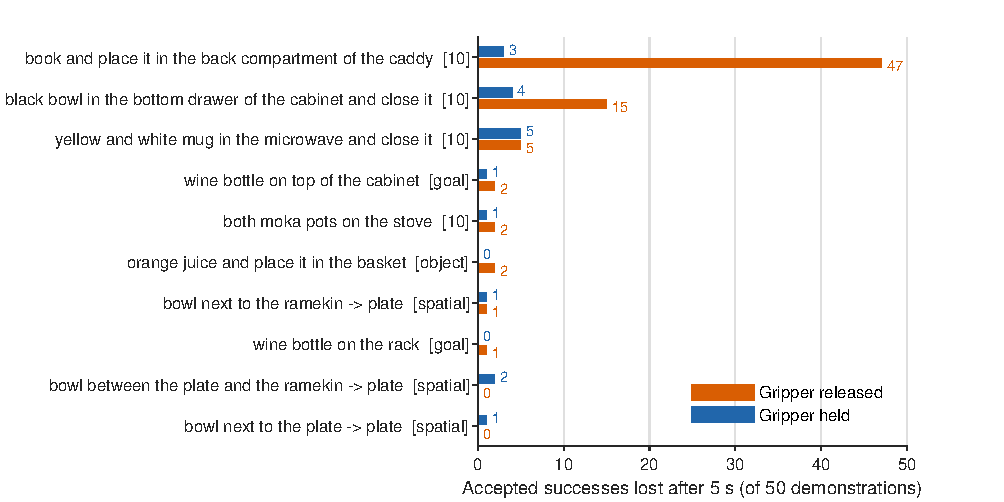
\includegraphics[width=0.86\textwidth]{fig_lost_by_task.pdf}
\caption{Accepted successes that no longer satisfy the predicate after 5\,s, per task, for the ten tasks with at least one such case. Suite in brackets. Each task has 50 demonstrations.}
\label{fig:tasks}
\end{figure*}

\subsection{A predicate that holds in the air and fails at rest}
\label{sec:book}
The goal of the task ``pick up the book and place it in the back compartment of the caddy'' is \pred{In}(\texttt{black\_book\_1}, \texttt{desk\_caddy\_1\_back\_contain\_region}). Under release it loses 47 of 50 accepted successes; under hold, 3.

We examined eight of its demonstrations state by state. Seven end with the gripper commanded closed and the book held at a height of 0.94 to 1.03\,m, inside the region. Under hold, the book stays in the gripper and the predicate remains true for all 100 steps. Under release, in six of the eight the book descends 5 to 13\,cm, shifts at most 2.4\,cm horizontally, keeps its orientation, and comes to rest at a height of 0.899\,m. In the first demonstration the predicate is true at 0.941\,m and at 0.918\,m, and false from 0.899\,m onward; it does not recover.

Renders of three demonstrations from two viewpoints confirm the reading (Fig.~\ref{fig:book}). In two of them the predicate is true while the book is held by the gripper and protrudes above the compartment, and false once the gripper has withdrawn and the book stands upright on the floor of the same compartment, fully inside it. In the third, the one whose predicate stays true, the released book does not drop: it remains perched on the upper edge of the caddy, leaning, at a height of 1.008\,m. In these three cases the predicate is true exactly when the book is not seated in the compartment. The containment box of this region evidently lies at the height of the caddy's rim. The renders were inspected by the authors and are not blind labels.

\begin{figure*}[t]
\centering
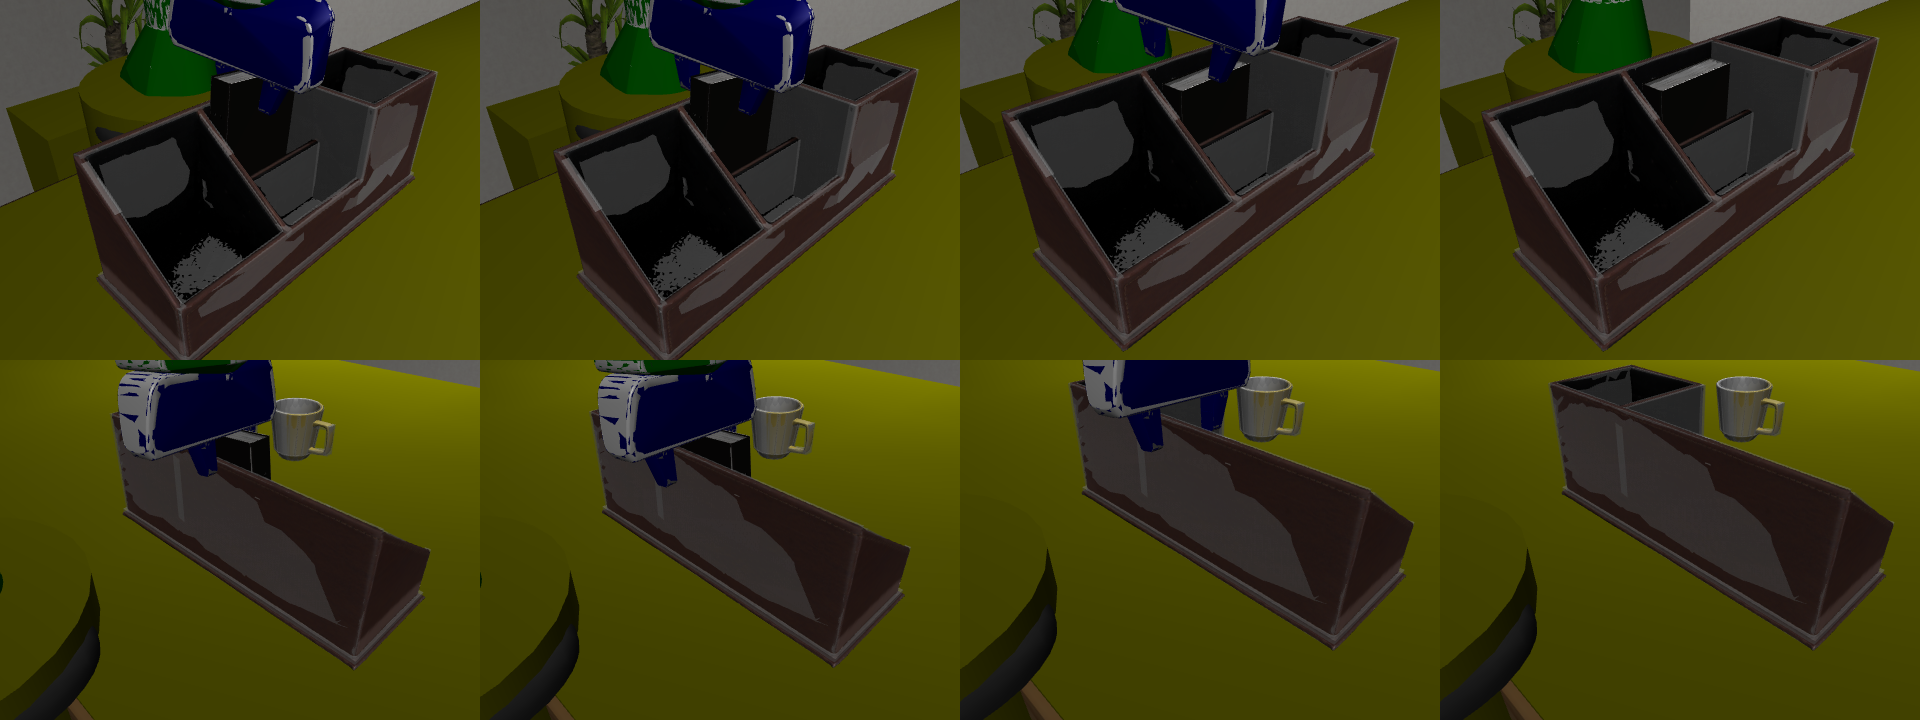
\includegraphics[width=\textwidth]{fig_book_demo0.png}\\[2pt]
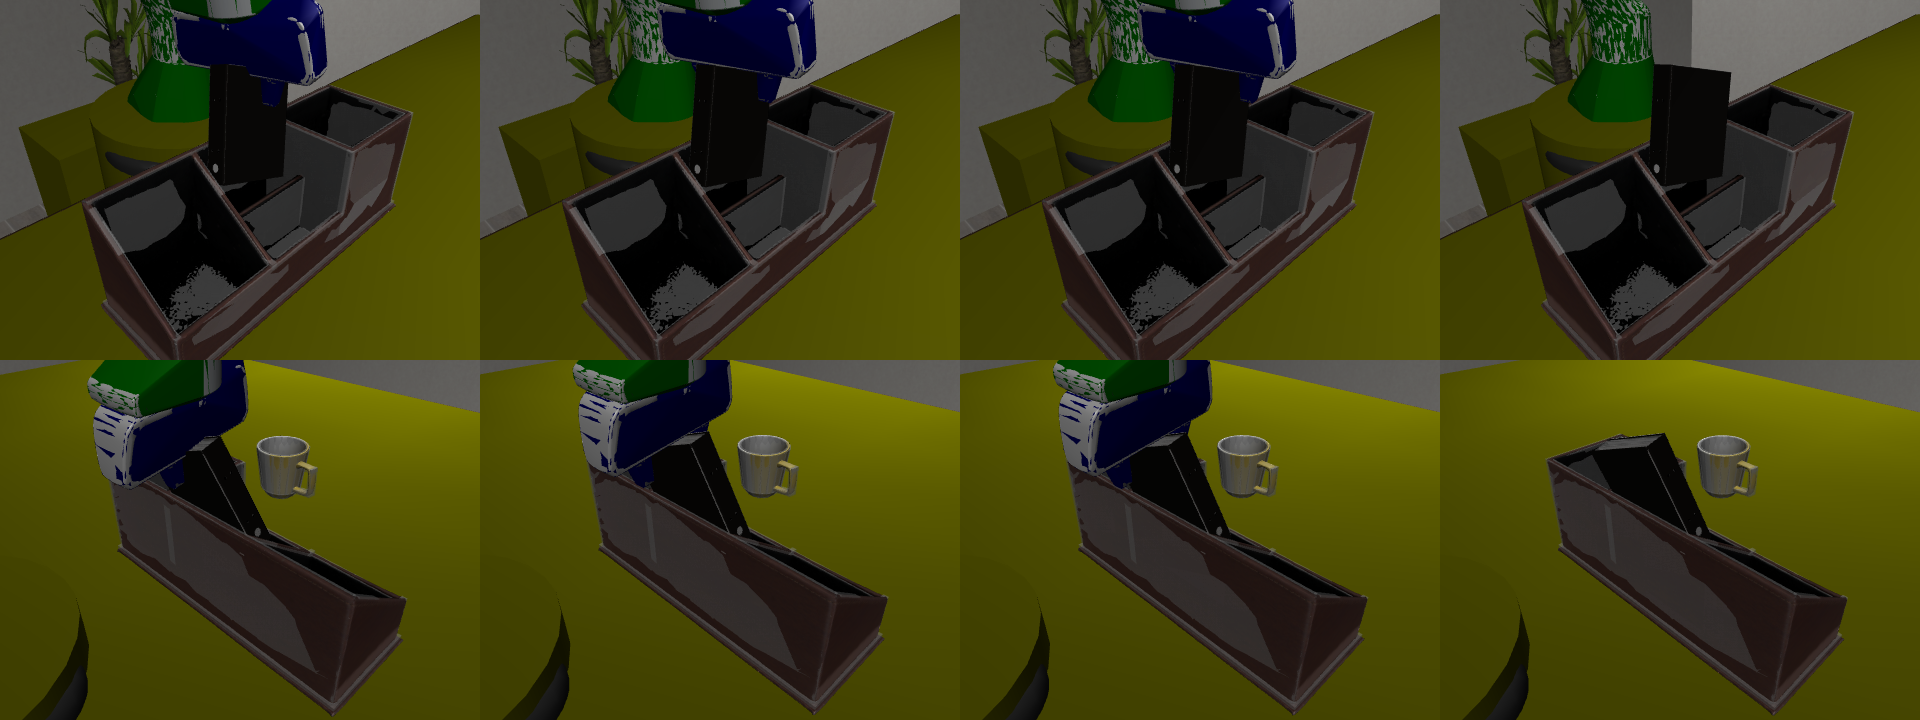
\includegraphics[width=\textwidth]{fig_book_demo2.png}
\caption{The book task under the release protocol, two viewpoints per demonstration; columns are the last logged state and extension steps 10, 20 and 100. \textbf{Top two rows} (demonstration 0): the predicate is \emph{true} in the two left columns, where the gripper holds the book above the compartment, and \emph{false} in the two right columns, where the book stands inside it. \textbf{Bottom two rows} (demonstration 2): the released book stays perched on the rim of the caddy and the predicate is \emph{true} in all four columns.}
\label{fig:book}
\end{figure*}

\subsection{Persistence windows reject stable placements}
No demonstration fails a 10-step window, as expected, since acceptance required one. A 30-step window rejects 58 demonstrations under release and 14 under hold, and every one of them is also lost; it misses 17 and 4 lost successes respectively. A 100-step window rejects every lost success and, in addition, 36 demonstrations under release and 41 under hold whose success is intact at the end. These are placements whose predicate flickers. Among episodes that are not lost, a 100-step window thus produces a false rejection in 36 of 1{,}925 (1.9\%) and 41 of 1{,}982 (2.1\%). Flicker is most frequent for contact-based \pred{On} goals (Fig.~\ref{fig:flicker}).

\begin{figure}[t]
\centering
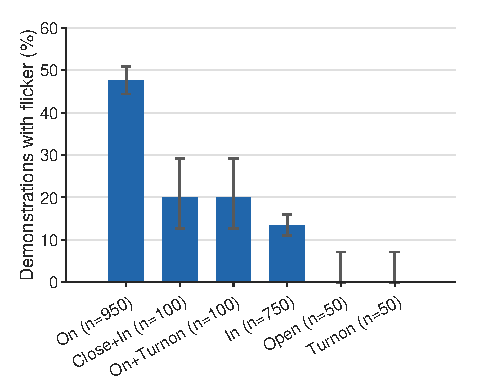
\includegraphics[width=0.92\columnwidth]{fig_flicker_by_class.pdf}
\caption{Share of demonstrations in which the predicate turns false at least once after first turning true, by goal-predicate class (release protocol). Bars show exact 95\% intervals.}
\label{fig:flicker}
\end{figure}

\section{Discussion}

\paragraph{What the benchmark's success means.} In LIBERO, success is the event that a geometric condition was met at some instant. For most tasks that event is followed by a stable final state, so the distinction is harmless for skilled demonstrations. For a minority of tasks it is not, and for the book task the event and the intended final state are different things.

\paragraph{Why demonstrations are the conservative case.} A human demonstrator places deliberately, and the collection rule already enforced a 10-step hold. A learned policy is graded on one step, and is trained on demonstrations that end as soon as the hold completes, often before release. We therefore expect the gap between first-hit success and durable success to be no smaller for policies than the 0.9\% to 3.75\% measured here, and to grow for policies that approach the goal region without completing a placement. This expectation is untested: it requires policy rollouts.

\paragraph{The post-success protocol is part of the metric.} Releasing the gripper instead of holding changes the pooled loss from 0.90\% to 3.75\%, and for the book task from 3 to 47 of 50. Any stricter grader that looks beyond the first hit must state what the robot does in that interval. An evaluation that lets the policy continue will produce a third answer.

\paragraph{Strict grading needs a debounce, not a long window.} The contact-based \pred{On} predicate turns false again in 48\% of demonstrations, nearly all of which end well. A 100-step window therefore rejects about 2\% of intact successes, while a 30-step window misses about a quarter of the lost ones. A grader that asks for the goal at the end of a fixed interval after release, or for a majority of steps within a window, would separate the two cases that a consecutive-step rule conflates. We have not yet evaluated such a grader.

\paragraph{Report uncertainty at the level at which errors occur.} Sixty-three percent of the loss sits in one task. An interval computed over episodes reports a precision the design does not have. Benchmark papers that pool over tasks should resample tasks.

\paragraph{Recommendations for users of LIBERO.}
\begin{enumerate}
\item Report per-task success alongside suite averages; the suite average hides task-specific predicate behaviour.
\item Treat results on the book-in-caddy task with caution, and examine the two \pred{In}+\pred{Close} tasks before relying on them.
\item When restoring simulator states, refresh the controller before stepping, and do not regenerate states by open-loop action replay across simulator versions.
\item When a claim is a null (``error below 1\%''), size the sample for it: 368 episodes with zero events per unit of analysis at the 95\% level.
\end{enumerate}

\section{Limitations and Threats to Validity}
\label{sec:limits}

\begin{enumerate}
\item \textbf{No human reference.} ``Lost'' compares the predicate with itself 5\,s later. A lost success may be a correct final state that the predicate rejects, as in the book task, or a real failure. Outside the three rendered demonstrations the two are not separated.
\item \textbf{Demonstrations, not policies.} Nothing here measures the error in a reported policy success rate. Policies differ from demonstrators in skill, in when they release, and in what they do after the goal is met.
\item \textbf{Simulator versions.} States are restored exactly, but the 100 extension steps run on MuJoCo 3.2.3 and robosuite 1.4.0, which may differ from the recording versions. The open-loop replay drift we observed shows that version differences are not negligible.
\item \textbf{Scripted protocols.} Both post-success protocols are artificial. The release protocol retreats upward regardless of the task, which may disturb articulated objects the gripper is still touching; this may contribute to the losses in the two \pred{In}+\pred{Close} tasks.
\item \textbf{Thresholds.} The screening uses fixed velocity thresholds and a 10-step window; no sensitivity sweep has been run.
\item \textbf{Sample size per task.} With 50 demonstrations, zero observed losses bounds a task's rate only below 7.1\% at the 95\% level. Task-level claims are limited to the tasks with large effects.
\item \textbf{One benchmark.} LIBERO-PRO, LIBERO-Plus, LIBERO-X, RoboCasa and others are not covered. The mechanism lies in LIBERO's shared environment code, so derived benchmarks that reuse it would inherit it, but that has not been measured.
\item \textbf{Related work read from abstracts.} Overlap with \cite{wang2026liberox}, \cite{valle2026mango} and \cite{zhou2026simuguard} may be larger than stated.
\end{enumerate}

\section{Conclusion}

LIBERO declares success at the first instant a geometric condition holds, with no requirement that the object be released, at rest or still in place a moment later. On the benchmark's own 2{,}000 demonstrations this is mostly harmless: 0.90\% of accepted successes are gone after 5\,s with the gripper held and 3.75\% with it released. The exceptions are few and large. One task supplies 63\% of the loss, and its predicate accepts the object while it is held above the compartment and rejects it once it stands inside. The predicate also flickers in 30\% of demonstrations, which makes consecutive-step persistence an unreliable strict grader.

The study the field needs next is the one this paper does not contain: the same extended-rollout protocol applied to strong and mid-performing policies on standard and perturbed suites, with human labels as the reference and intervals resampled over tasks. The harness, graders and estimators for it are in place.

\section*{Reproducibility}
Code: \url{https://github.com/Makuma102/predicate-audit}. Data: the official LIBERO demonstration files (\url{https://huggingface.co/datasets/yifengzhu-hf/LIBERO-datasets}). The pipeline is: \texttt{download\_libero\_suite}, \texttt{build\_libero\_taxonomy}, \texttt{run\_demo\_terminal\_audit} (MATLAB R2019b or newer, no toolbox); \texttt{sim\_shim/replay\_demos.py} (Python 3.8, robosuite 1.4.0, MuJoCo 3.2.3, no rendering needed); \texttt{run\_pooled\_summary} and \texttt{make\_figures} (MATLAB). Bootstrap intervals use seed 0 and 5{,}000 resamples.

\begin{thebibliography}{99}\small
\bibitem{jiang2026benchmarking} T.~Jiang, X.~Tan, S.~Wheeler, et al. What are we actually benchmarking in robot manipulation? arXiv:2606.04233, 2026.
\bibitem{liu2023libero} B.~Liu, Y.~Zhu, C.~Gao, et al. LIBERO: Benchmarking knowledge transfer for lifelong robot learning. arXiv:2306.03310, 2023.
\bibitem{wang2026liberox} G.~Wang, C.~Zhang, Q.~Liu, et al. LIBERO-X: Robustness litmus for vision-language-action models. arXiv:2602.06556, 2026.
\bibitem{zhou2025liberopro} X.~Zhou, Y.~Xu, G.~Tie, et al. LIBERO-PRO: Towards robust and fair evaluation of vision-language-action models beyond memorization. arXiv:2510.03827, 2025.
\bibitem{fei2025liberoplus} S.~Fei, S.~Wang, J.~Shi, et al. LIBERO-Plus: In-depth robustness analysis of vision-language-action models. arXiv:2510.13626, 2025.
\bibitem{valle2026mango} P.~Valle, S.~Ali, A.~Arrieta, et al. MANGO: Automated multi-agent test oracle generation for vision-language-action models. arXiv:2606.24815, 2026.
\bibitem{fan2026safevla} J.~Fan, W.~Xu, Z.~Wang, et al. SafeVLA-Bench: A benchmark for the success-safety gap in vision-language-action models. arXiv:2606.00773, 2026.
\bibitem{navasardyan2026failbench} Z.~Navasardyan, T.~Danielyan, H.~Davtyan. FailBench: How reliable are VLMs at judging robot task success? arXiv:2609.03611, 2026.
\bibitem{zhou2026simuguard} A.~Zhou, J.~Wu, X.~Zhou, et al. When the simulator fails, not the policy: Auditing contact artifacts in simulated robot benchmarks. arXiv:2610.41857, 2026.
\bibitem{bedi2026silent} A.~Bedi. How visible are silent manipulation failures? An observability study of false-success detection in simulated robot episodes. arXiv:2606.03134, 2026.
\bibitem{nasiriany2024robocasa} S.~Nasiriany, A.~Maddukuri, L.~Zhang, et al. RoboCasa: Large-scale simulation of everyday tasks for generalist robots. arXiv:2406.02523, 2024.
\bibitem{clopper1934} C.~J. Clopper and E.~S. Pearson. The use of confidence or fiducial limits illustrated in the case of the binomial. \emph{Biometrika}, 26, 1934.
\bibitem{davison1997} A.~C. Davison and D.~V. Hinkley. \emph{Bootstrap Methods and their Application}. Cambridge University Press, 1997.
\end{thebibliography}

\end{document}
